% ============================================================
%  nature.tex — 《数学地图》排版样式（对标 Nature 的清爽编辑风）
%  由 pandoc --include-in-header 注入。配色、标题、页眉页脚、图注。
% ============================================================
\usepackage{xcolor}
\definecolor{natblue}{HTML}{0B5394}
\definecolor{natdark}{HTML}{12303F}
\definecolor{natgray}{HTML}{5A6672}
\definecolor{natlight}{HTML}{EEF3F7}
\definecolor{natrule}{HTML}{D5DDE5}
\definecolor{nataccent}{HTML}{C0392B}

\usepackage{titlesec}
\usepackage{titletoc}
\usepackage{fancyhdr}
\usepackage{caption}
\usepackage{enumitem}
\usepackage{array}
\usepackage{colortbl}
\usepackage{tcolorbox}
\tcbuselibrary{skins,breakable}

\graphicspath{{book/}{./}}

% 超链接配色（若 pandoc 未加载 hyperref 则补上）
\makeatletter
\@ifpackageloaded{hyperref}{}{\usepackage{hyperref}}
\makeatother
\hypersetup{colorlinks=true,linkcolor=natblue,urlcolor=natblue,citecolor=natblue}

% ---------- 章节标题 ----------
\titleformat{\chapter}[hang]
  {\normalfont\sffamily\bfseries\color{natblue}\Huge}
  {\colorbox{natblue}{\color{white}\sffamily\bfseries\thechapter}\hspace{0.55em}}
  {0pt}{\Huge}
  [\vspace{0.22em}{\color{natrule}\hrule height 1pt}]
\titlespacing*{\chapter}{0pt}{4pt}{26pt}

\titleformat{\section}
  {\normalfont\sffamily\bfseries\large\color{natdark}}{\thesection}{0.6em}{}
\titleformat{\subsection}
  {\normalfont\sffamily\bfseries\normalsize\color{natblue}}{\thesubsection}{0.5em}{}
\titleformat{\subsubsection}
  {\normalfont\sffamily\bfseries\small\color{natgray}}{}{0em}{}

% ---------- 页眉页脚 ----------
\providecommand{\booktitle}{数学地图}
\pagestyle{fancy}
\fancyhf{}
\renewcommand{\headrulewidth}{0.4pt}
\renewcommand{\footrulewidth}{0pt}
\fancyhead[L]{\sffamily\small\color{natgray}\booktitle}
\fancyhead[R]{\sffamily\small\color{natgray}\leftmark}
\fancyfoot[C]{\sffamily\small\color{natgray}\thepage}
\fancypagestyle{plain}{\fancyhf{}\renewcommand{\headrulewidth}{0pt}%
  \fancyfoot[C]{\sffamily\small\color{natgray}\thepage}}

% ---------- 图注 ----------
\captionsetup{font={small,sf},labelfont={bf,color=natblue},labelsep=quad,skip=6pt}
\captionsetup[figure]{name=图}
\captionsetup[table]{name=表}
\setlength{\intextsep}{12pt}
\setlength{\textfloatsep}{18pt}

% ---------- 版式细节 ----------
\setlength{\parskip}{0.45em}
\setlength{\parindent}{0pt}
\setlist[itemize]{topsep=2pt,itemsep=1.5pt,parsep=0pt}
\setlist[enumerate]{topsep=2pt,itemsep=1.5pt,parsep=0pt}

% 引用块（Obsidian callout 转换而来）：浅蓝左边线
\renewenvironment{quote}
  {\begin{tcolorbox}[enhanced,breakable,colback=natlight,colframe=natlight,
     left=8pt,right=8pt,top=6pt,bottom=6pt,boxrule=0pt,
     borderline west={2.5pt}{0pt}{natblue}]}
  {\end{tcolorbox}}

% ---------- 封面 ----------
\makeatletter
\providecommand{\booksubtitle}{}
\renewcommand{\maketitle}{%
  \begin{titlepage}%
  \thispagestyle{empty}%
  \centering
  \vspace*{2.0cm}
  {\sffamily\bfseries\color{natblue}\fontsize{44}{50}\selectfont \@title\par}
  \vspace{0.45cm}
  {\sffamily\color{natgray}\fontsize{18}{24}\selectfont \booksubtitle\par}
  \vspace{0.5cm}
  {\color{natrule}\rule{0.46\textwidth}{1.1pt}\par}
  \vspace{1.1cm}
  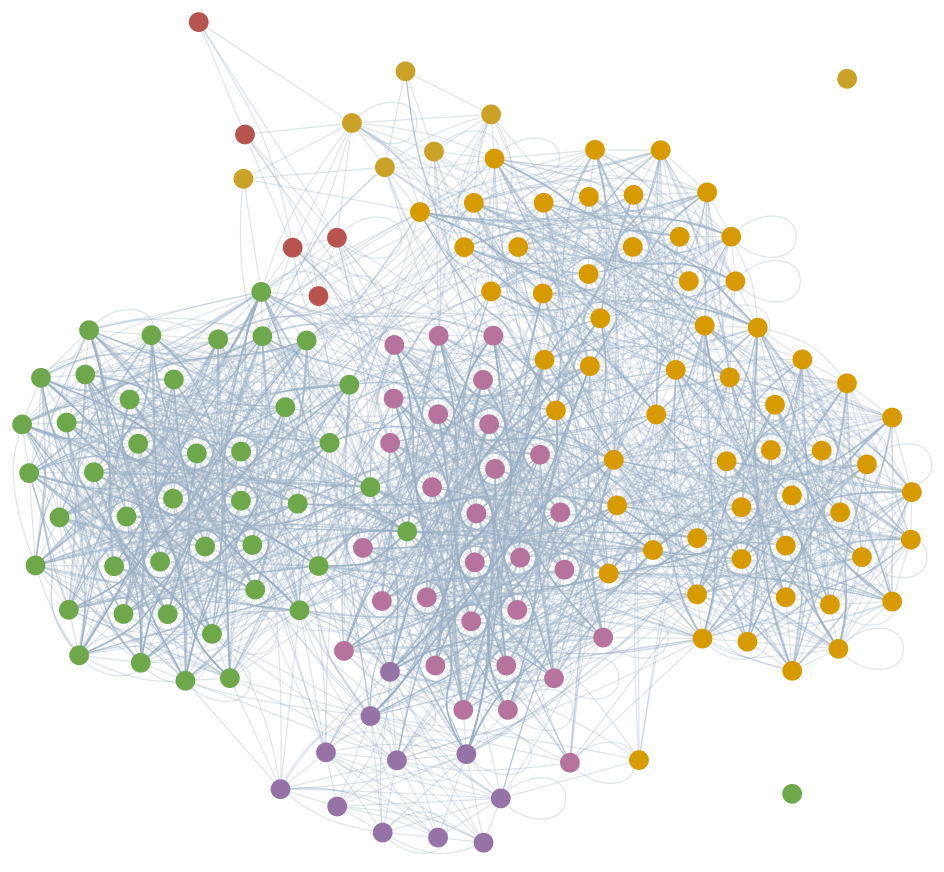
\includegraphics[width=0.74\textwidth]{figures/fig-network.png}\par
  \vfill
  {\sffamily\large\color{natdark}\@author\par}
  \vspace{0.28cm}
  {\sffamily\small\color{natgray}\@date\par}
  \vspace{1.6cm}
  \end{titlepage}%
  \clearpage
}
\makeatother
